\documentclass[a4paper,10pt,notitlepage,pdftex,headsepline]{scrartcl}

\usepackage{a4wide}
\usepackage{cmap} % чтобы работал поиск по PDF
\usepackage[utf8]{inputenc}
\usepackage[russian]{babel}
\usepackage[T2A]{fontenc}

\usepackage{textcase}
\usepackage[pdftex]{graphicx}

\pdfcompresslevel=9 % сжимать PDF
\usepackage{pdflscape} % для возможности альбомного размещения некоторых страниц
\usepackage[pdftex]{hyperref}
% настройка ссылок в оглавлении для pdf формата
\hypersetup{unicode=true,
            pdftitle={ДКР по ЧМ №1},
            pdfauthor={Погода Михаил},
            pdfcreator={pdflatex},
            pdfsubject={},
            pdfborder    = {0 0 0},
            bookmarksopen,
            bookmarksnumbered,
            bookmarksopenlevel = 2,
            pdfkeywords={},
            colorlinks=true, % установка цвета ссылок в оглавлении
            citecolor=black,
            filecolor=black,
            linkcolor=black,
            urlcolor=blue}

\usepackage{amsmath}
\usepackage{amssymb}
\usepackage{moreverb}
%for \includepdf
%\usepackage{pdfpages}

\author{Михаил Погода}
\title{Домашняя контрольная работа №1 по численным методам}
\date{\today}
\begin{document}
\maketitle

\section{Задание}
\begin{figure}[hc]
\begin{tabular}{c|c|c|c|c|c|c|c|c|c|c|}
$x$ & $1.415$ & $1.420$ & $1.425$ & $1.430$ & $1.435$ & $1.440$ & $1.445$ & $1.450$ & $1.455$ & $1.460$\\
\hline
$y$ & $0.880$ & $0.889$ & $0.890$ & $0.891$ & $0.892$ & $0.893$ & $0.894$ & $0.895$ & $0.896$ & $0.897$
\end{tabular}
\end{figure}
\subsection{Метод Эйткена}
Посчитать значение функции в точке $x_1 = 1.4167$.

Запрограммировав алгоритм метода Эйткена (см.~Приложение), получим $y_1 = 0.8856$.
\subsection{Метод Лагранжа}
Посчитать значение функции в точке $x_2 = 1.424$ с точностью до $0.001$.

Запрограммировав алгоритм метода Лагранжа (см.~Приложение), учитывая то, что нам достаточно точности $0.001$, получим $y_2 = 0.8898$.
Проверка точности заключается в том, что сравнивается значение в точке $x_2$ полиномов $n$-ой и $(n+1)$-ой степени. Если разница между этими значениями меньше, чем $0.001$, значит мы достигли нужной точности, и следующие шаги алгоритму не нужно делать. В этом примере, достаточным оказалась интерполяция полиномом 2 степени.
\subsection{Методы основанные на многочлене Ньютона}
\subsubsection{Задание 1}
Посчитать значение функции в точке $x_3 = 1.436$.

Т.\,к. точка $x_3$ находится около середины таблицы функции, и шаг этой таблицы одинаков, можно воспользоваться формулой Стирлинга. Запрограммировав её (см.~Приложение), получим значение $y_3 = 0.8921$.
\subsubsection{Задание 2}
Посчитать значение функции в точке $x_4 = 1.461$.

Т.\,к. точка $x_4$ больше всех точек в нашей таблице, то экстраполировать функцию вправо мы можем с помощью второй формулы Ньютона. Запрограммировав её (см.~Приложение), получим значение $y_4 = 0.8975$.
\newpage
\section*{Приложение}
\subsection*{Исходный текст для GNU Octave (совместим с Matlab)}
\begin{small}
\listinginput{1}{nummethods.m}
\end{small}
\newpage
\subsection*{График функции}
\begin{figure}[hc]
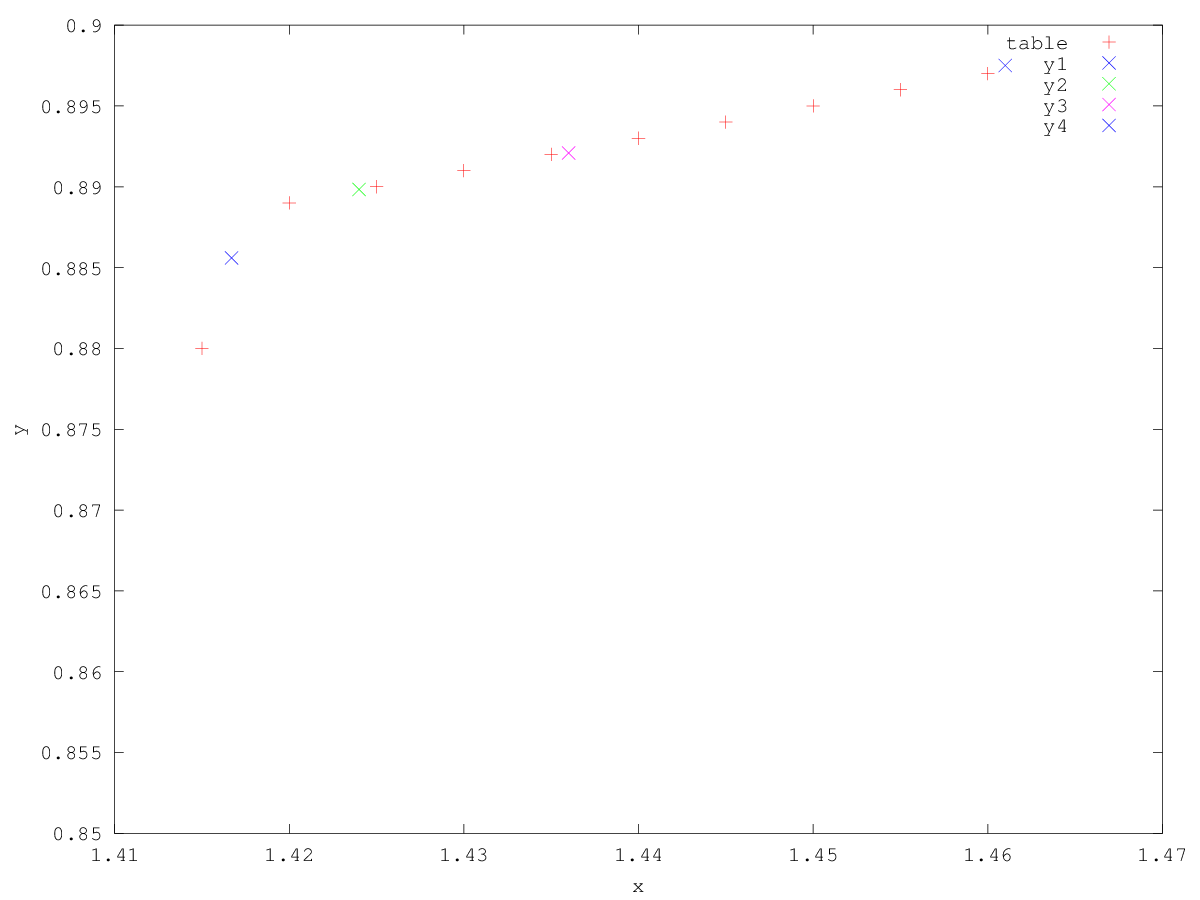
\includegraphics[scale=0.75]{1.png}
\end{figure}
\end{document}